\documentclass[../Main/Knit.tex]{subfiles}
\newpage

\subsection{Lab Pipeline}

In brief, the Iso-Seq protocol involved converting total RNA transcripts to full-length complementary DNA (cDNA) using the Clontech SMARTer PCR cDNA synthesis kit, which was then subsequently amplified and purified to generate double-stranded cDNA. The cDNA was then constructed to a SMRT bell library for sequencing. Size selection was not performed with full-length transcript detection of up to 4 kB. For targeted sequencing using IDT probes, all the steps in the Iso-Seq protocol are the same with an additional step of target capture post ds-DNA amplification and pre SMRT bell library, and usage of barcodes to allow multiplexing. 

\begingroup
\parindent=0em
\etocsettocstyle{\rule{\linewidth}{\tocrulewidth}\vskip0.5\baselineskip}{\rule{\linewidth}{\tocrulewidth}}
\etocsetnexttocdepth{5}
\localtableofcontents 
\endgroup

\subsubsection{CDNA synthesis}
\label{section:ch2_cDNA_synthesis_explanation} 
As part of the official Iso-Seq protocol, SMARTer PCR cDNA Synthesis Kit (Clontech) was used to convert extracted total RNA to complementary DNA by first strand cDNA synthesis, as outlined in Figure X. In brief, the polyA+ tails of RNA transcripts is first primed by a modified oligo (dT) primer, transcribed by SMARTScribe Reverse Transcriptase to generate a first single-stranded DNA, which is then diluted and subsequently amplified \cite{Ramskold2012}. All reagents were provided with the kit, except for the Pacific Bioscience’s barcodes, with all reagents and consumables used being sterile and DNAse and RNAse free. In order to sequence samples simultaneously (“multiplex”), as exploited for targeted sequencing, unique barcoded oligo (dT) primer was used in place of the standard oligo (dT) primer (Table \ref{tab:barcode_primers}). With new Sequel system, cDNA can be sequenced without size selection. 

While this kit is advantageous in preferentially enriching for full-length cDNA sequences, as a template switching oligo is required to ensure complete reverse transcription, it cannot differentiate between intact and truncated RNA; which, present in poor-quality samples will be amplified as a potential source of contamination in the final cDNA library. One alternative is to exploit the 5’-cap that is present only in intact RNA and not truncated RNA (5-cap refers to the addition of 7-methylguanosine to the 5’-end of mRNA during transcription, to protect nascent mRNA from degradation and assist in protein translation). Alternative reverse transcriptase have been explored that only converts 5’capped mRNAs to cDNA, however, these have been found to negatively affect read length on the ONT platform (Cartolano et al. 2016). An alternative method, Full-Length cDNA Amplification (Teloprime), relies on a double-stranded adapter that recognises and ligates to the 5’cap at the end of first strand synthesis (Section X, Chapter 2)(\cite{Cartolano2016}). 

For this thesis, 200ng of total RNA was used for each sample for consistency and to ease downstream analyses. 

\begin{landscape}
The general structure of barcoded oligo-dT primer is as follows:
\\
\\
\hangindent=5cm \textcolor{RedOrange}{Primer Sequence} \hspace{2cm}   \textcolor{ForestGreen}{16-bp barcode}   \hspace{4cm} \textcolor{RoyalBlue}{oligo-dT}
\begin{center}
5'\textcolor{RedOrange}{AAGCAGTGGTATCAACGCAGAGTAC}\textcolor{ForestGreen}{tcagacgatgcgtcat}\textcolor{RoyalBlue}{TTTTTTTTTTTTTTTTTTTTTTTTTTTTTTVN3’}
\end{center}

	
\begin{table}[ht]
	\begin{tabularx}{1.45\textwidth}{ll}
		\toprule
		Barcode Name & Sequence                                                                  \\ \midrule
		Barcode 1    & AAGCAGTGGTATCAACGCAGAGTACCACATATCAGAGTGCGTTTTTTTTTTTTTTTTTTTTTTTTTTTTTTVN \\
		Barcode 2    & AAGCAGTGGTATCAACGCAGAGTACACACACAGACTGTGAGTTTTTTTTTTTTTTTTTTTTTTTTTTTTTTVN \\
		Barcode 3    & AAGCAGTGGTATCAACGCAGAGTACACACATCTCGTGAGAGTTTTTTTTTTTTTTTTTTTTTTTTTTTTTTVN \\
		Barcode 4    & AAGCAGTGGTATCAACGCAGAGTACCACGCACACACGCGCGTTTTTTTTTTTTTTTTTTTTTTTTTTTTTTVN \\
		Barcode 5    & AAGCAGTGGTATCAACGCAGAGTACCACTCGACTCTCGCGTTTTTTTTTTTTTTTTTTTTTTTTTTTTTTTVN \\
		Barcode 6    & AAGCAGTGGTATCAACGCAGAGTACCATATATATCAGCTGTTTTTTTTTTTTTTTTTTTTTTTTTTTTTTTVN \\
		Barcode 7    & AAGCAGTGGTATCAACGCAGAGTACTCTGTATCTCTATGTGTTTTTTTTTTTTTTTTTTTTTTTTTTTTTTVN \\
		Barcode 8    & AAGCAGTGGTATCAACGCAGAGTACACAGTCGAGCGCTGCGTTTTTTTTTTTTTTTTTTTTTTTTTTTTTTVN \\
		Barcode 9    & AAGCAGTGGTATCAACGCAGAGTACACACACGCGAGACAGATTTTTTTTTTTTTTTTTTTTTTTTTTTTTTVN \\
		Barcode 10 & AAGCAGTGGTATCAACGCAGAGTACACGCGCTATCTCAGAGTTTTTTTTTTTTTTTTTTTTTTTTTTTTTTVN \\ \bottomrule
	\end{tabularx}
\captionsetup{justification=raggedright,width=1.5\textwidth}
\caption[Barcoded Oligo-dT Primers for targeted transcriptome sequencing]%
{\textbf{Barcoded oligo-dT primers were used for multiplexing samples in targeted transcriptome sequencing}. Each of the barcoded primers contain the same 5' primer sequence and oligo-dT for reverse transcription of first strand cDNA synthesis using Clontech kit SMARTer PCR cDNA Synthesis Kit. The different internal 16bp sequence allows tagging and differentiation of samples in the same sequencing run. The barcodes are recommended from official PacBio's multiplex protocol.}
\label{tab:barcode_primers}
\end{table}
\end{landscape}

\subsubsection{PCR optimisation and DNA Amplification}
To minimise PCR bias (under or over-amplification), which can result in under or over representation of the different cDNA library size, the optimal number of PCR cycles for amplification of first-strand synthesis products was determined (Figure X). As described in Section X (Chapter 2), 5uL PCR aliquots were collected every two cycles (cycle 10, 12, 14, 16, 18) and run on a 1.5\% Agarose gel electrophoresis. With 200ng total input of total RNA, cycles 14 – 15 were selected for large scale amplification across all the mouse samples to generate sufficient amount of double-stranded cDNA product for SMRTbell library construction (Figure X). 

\subsubsection{Polymerase Chain Reaction (PCR)}
\label{section:ch2_PCR_explanation} 
To generate sufficient DNA for sequencing, single-stranded DNA was amplified using Polymerase Chain Reaction (PCR\nomenclature{PCR}{Polymerase Chain Reaction}), a well-established method of generating multiple copies of the same DNA sequence. Mimicking natural DNA replication, this relies on a thermostable DNA polymerase, a set of primers specific to the region of interest, and a cocktail of various other components required for polymerisation (deoxynucleotides\nomenclature{dNTPs}{Deoxynucleotides} , buffers). This reaction is then subjected to a series of heating and cooling steps: 
\begin{enumerate}
	\item Denaturation at 96C, to separate any double-stranded DNA 
	\item Annealing, typically between 55 to 65C, for the binding of primers to the complementary sequences on the single-stranded DNA; the specific annealing temperature is dependent on the primer sequence. 
	\item Extension at 72C to allow the polymerase to extend the primers, consequently synthesising a new complementary DNA strand using dNTPs
\end{enumerate} 
These three steps are then repeated for a number of times, "cycles", for an exponential generation of the DNA template of interest.

Single-stranded DNA generated from SMARTer PCR synthesis kit in the official Iso-Seq protocol was amplified by PCR using PrimeSTAR GXL DNA Polymerase (ClonTech). Also performed for targeted sequencing. 


\subsubsection{Agarose Gel Electrophoresis}
\label{section:ch2_agarose_explanation}  
Agarose gel electrophoresis allows the separation of (double-stranded) DNA molecules based on its length. It is most commonly used to determine DNA quality and quantity, and assess the efficiency of molecular biology techniques such as PCR amplification. It works on the principle that by applying an electrical charge, negatively-charged DNA migrates through a gel matrix towards the positive anode at a rate dependent on DNA size: smaller DNA fragments migrate faster, and thus move further through the gel within a specific time frame. The separated DNA can be then visualised using a fluorescent dye that intercalates into the DNA structure and fluoresces under ultraviolet light. 

For this thesis, visualisation of DNA through gel electrophoresis was required primarily for optimising the number of PCR cycles for amplification, and for validating transcripts identified from Iso-Seq in Chapters X. A 1.5\% agarose gel was made, with the separated DNA visualised using ethidium bromide on XXXX, as detailed in Section \ref{Isoseq_Protocol_running_agarose_gel}.


\subsubsection{AMPure Bead Purification} 
Post large scale amplification, the resulting PCR product was divided into two fractions and purified with 0.4X and 1X AMPure PB beads (PacBio), as described in Section X (Chapter 2).  In brief, ds-DNA was bound to the beads in either 1:1 or 1:0.4 ratio, which were then isolated on a magnetic rack, and washed with 70\% ethanol. DNA purification with 0.4x AMPure beads allows for enrichment of longer DNA fragments to provide a more representative library given that shorter fragments diffuse quicker into ZMW and are more likely to be sequenced. The ability to enrich for longer fragments is due to the preferential binding of beads to more negatively-charged, and subsequently larger molecular weight DNA, and thus displacement of shorter fragments.  Quantification and size distribution of each fraction was then determined using Qubit DNA High sensitivity assay (Invitrogen) and Bioanalyzer 2100 (Agilent), as described in Section X, Chapter X. Two fractions per sample were then recombined at equimolar quantities and library preparation performed using SMRTbell Template Prep Kit v1.0 (PacBio) (Figure X). 

The molarity was calculated by the following equation: 
\begin{equation}
\frac{concentration(\frac{ng}{ul})\times 10^6}{660(\frac{g}{mol}) \times average\:library\:size\:in\:bp\mbox{*}} = concentration\;in\; nM
\end{equation}
* the average library size was determined by the start and end point of the smear

\subsubsection{Bioanalyzer and Tapestation}
\label{section:ch2_bioanalyzer} 
ScreenTape and Bioanalyzer assays are commonly used to provide accurate assessment of nucleic acid quality and size, prior to proceeding with downstream experiments. As an automative alternative to agarose gel electrophoresis, both assays similarly take advantage of nucleic acid's inclination to migrate in response to an electrical field.
While the Bioanalyzer assay is more sensitive than the ScreenTape assay, it is more expensive to run as it uses a chip consisting of 12 sample wells rather than independent lanes on the ScreenTape. 

For this thesis, most of the assessments of DNA quality in the Iso-Seq and ONT protocol were performed on the DNA 12000 Kit (Agilent) on the 2100 Bioanalyzer assay for accurate determination of library molarity (Section X). However, the D5000 ScreenTape (Agilent) was used in a few of the quality control steps where it is optional to assess for DNA quality (Section X).

RNA extracted by Dr Isabel Castanho was also run on RNA ScreenTape assay and the Bioanalyzer RNA analysis to provide accurate evaluation of RNA degradation; this is represented by a RNA Integrity Number (RIN\nomenclature{RIN}{RNA Integrity Number}) between 1 and 10, where 1 is indicative of high degradation, and 10 of low degradation and thus high integrity (Figure \ref{fig:bionalayzer_pics}). As a pre-requisite for good sequencing yield on Sequel and MinION, only samples with RIN $>$ 8 were selected for long-read sequencing on Iso-Seq and ONT protocol.

\spacetable
\begin{figure}[h]
	\centering
	\begin{subfigure}{0.4\linewidth}
		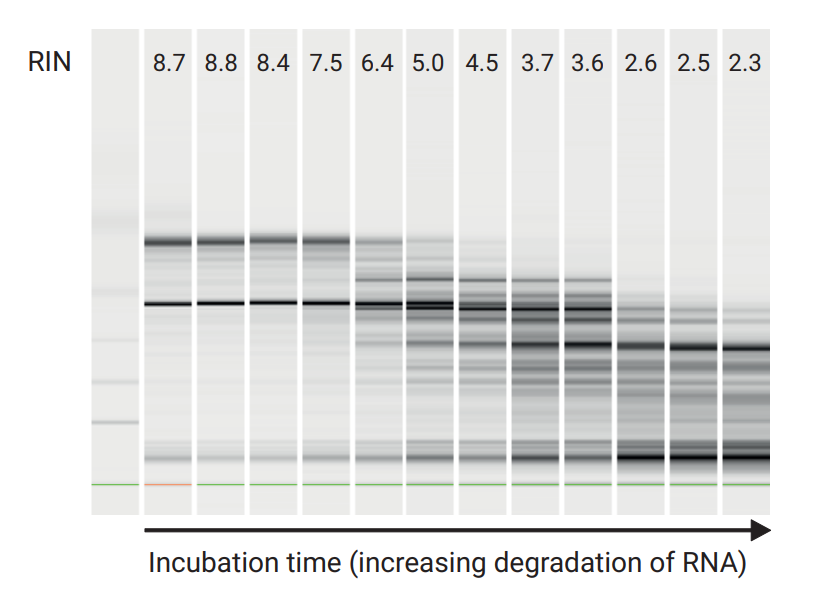
\includegraphics[width=\linewidth, height=0.21\textheight]{Pictures/RNA_degradation.png}
		\caption{Automated gel electrophoresis of RNA degradation}
	\end{subfigure}
	\hspace{2em}
	\begin{subfigure}{0.4\linewidth}
		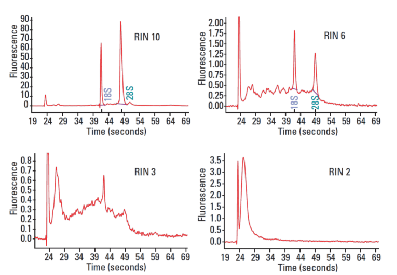
\includegraphics[width=\linewidth, height=0.21\textheight]{Pictures/RIN_range.png}
		\caption{Electropherogram of RNA degradation}
	\end{subfigure}
	\hspace{2em}
	\begin{subfigure}{0.4\linewidth}
		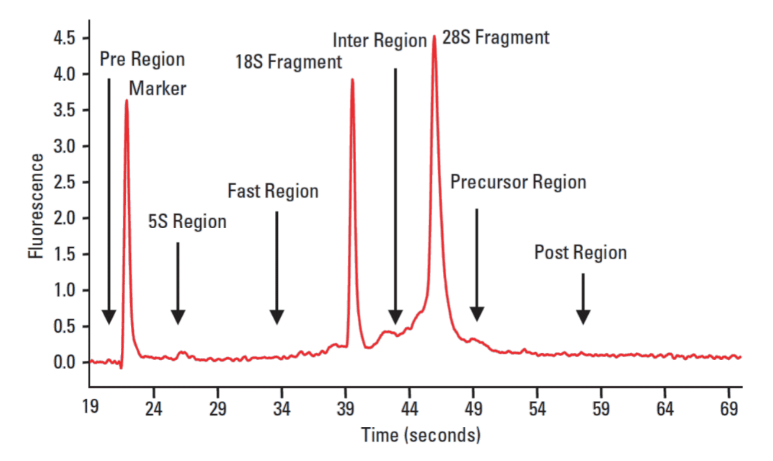
\includegraphics[width=\linewidth,
		height=0.21\textheight]{Pictures/RIN_regions.png}
		\caption{Electropherogram of regions that are indicative of RNA quality}
	\end{subfigure}
	\captionsetup{width=0.95\textwidth}
	\caption[Evaluation of RNA integrity with Bioanalyzer and Tapestation]%
	{\textbf{Evaluation of RNA integrity with Bioanalyzer and Tapestation}: Total RNA degradation can be observed by a shift towards shorter fragment size as depicted in Figure a, after prolonged incubation. The degree of degradation is represented by a RNA integrity number (RIN), ranging from intact (RIN = 10) to degraded (RIN = 2) RNA, and is calculated by the relative ratio of the fast region and 18S, 28S fragment (Figure c). Figures and legends are adapted from Mueller et al. 2016.}
	\label{fig:bionalayzer_pics}
\end{figure} 

\subsubsection{Qubit}
\label{section:ch2_qubit}   
Qubit assays allow accurate nucleic acid quantification by the selective binding of fluorescent Qubit dyes to double-stranded DNA (dsDNA\nomenclature{dsDNA}{double-stranded DNA}) or RNA, making it more sensitive and specific than UV absorbance used in NanoDrop 8000 spectrophotometer (Thermo Fisher Scientific). It is commonly performed to determine the average concentration of DNA or RNA prior to proceeding with downstream experiments. Many of the steps in the Iso-Seq protocol and ONT protocol thus require performing Qubit assays, particularly post bead purification, and are detailed in Section \ref{Isoseq_Protocol_qubit}.  

\subsubsection{Target Capture using IDT Probes} 
For targeted sequencing, we used the official PacBio protocol “cDNA Capture Using IDT
xGen® Lockdown Probes” (an adaptation of the official IDT protocol “xGen hybridisation capture of DNA libraries” ), which slotted as an additional step to the standard protocol between cDNA amplification and ligation. Enrichment of target genes involved hybridisation of dsDNA using pre-designed, complementary 5’ biotinylated DNA 120nt-long oligonucleotides (hereby referred as probes). The hybridised library fragments were then washed, isolated with magnetic streptavidin beads, amplified using Takara Hot-Start polymerase and then further purified with AMPure beads. After assessing the quality and quantity of the target cDNA using the bionanalyzer and qubit, SMRT Bell template preparation, primer and polymerase annealing were proceeded as per standard Iso-Seq protocol. Given the samples were multiplexed for targeted sequencing, the samples were first pooled in equal molarity before probe hybridisation.  


%*Modifications to the protocol: waiting times at room temperature during hybridisation, lid heat temperatures, method of washing beads at room temperature; all modifications are incorporated from official IDT protocol, post amplification clean-up for consistency  

\myparagraph{Selection of probes}
Probes were designed to a panel of 20 AD-associated genes: Bin1, Trem2, Cd33, Vgf, FynMapt, Trpa1, Picalm, Sorl1, Abca7, Snca, Apoe, Abca1, App, Ank1, Clu, Fus, Ptk2b, Rhbdf2, Tardbp. Two separate pools of the equal molar probes were created using the mouse genome (GRCm28/mm10) and human genome (GRCh37/hg19). While IDT provided a pre-designed set of probes to the target genes, many of them were found to overlap with the intronic regions of the target gene with contiguous coverage. 

Given that previous studies with targeted sequencing have found that the target gene can be successfully enriched with a few unique probes to the exonic regions, I manually assessed the list of probes for each target gene using the following criteria:
\begin{itemize}
	\item Ensured each exon in every gene is covered at least once (exons > 500bp has >1 probe) 
	\item Removed any probes to intronic regions
	\item Within each exon, removed any contiguous probes (as seen in the 1x tiling density) and ensured probes spaced 300-500bp (equivalent to 0.2x – 0.3x tiling density) 
	\item From the contiguous “cluster”, selected probes with the highest GC content (40-65\% GC content)/minimal number of blast hits 
\end{itemize}
The coverage of each target gene can be found in Appendix. 


\subsubsection{SMRT Bell Template Preparation}
As described in Section X (Chapter 2), DNA Damage and End Repair was performed on the pooled library to polish ends of fragments for ligation of blunt hairpin adapters, necessary to generate high quality library of closed, circular SMRTBell templates. Any abasic sites were filled-in, thymine dimers resolved, and deaminated cytosine are alkylated. 3’ overhangs were removed, whereas 5’ overhangs were filled-in by T4 DNA Polymerase and phosphorylated by T4 PNK. Following 1x AMPure purification of repaired dsDNA, hairpin adapters were then ligated to the blunt ends for up to 24hours. Any fragments failed to ligate were removed with exonuclease III and VII. The repaired, ligated SMRT bell library was then purified twice with 1x AMPure beads, and assessed with Qubit DNA High sensitivity assay (Invitrogen) and Bioanalyzer 2100 (Analyzer) before proceeding to primer annealing and polymerase binding (Figure X). 

\subsubsection{Primer Annealing and Polymerase Binding} 
Post ligation of hairpin adapters, sequencing primer and polymerase were bound to both ends of the SMRTbell templates. The primer and polymerase to template ratio was critical to minimise under or –over loading, thus the concentration was sample specific. 

Prior to XXX chemistry, MagBead Loading was only recommended for IsoSeq SMRTbell libraries, whereas Diffusion Loading was recommended for all other applications with insert sizes from 
250 – 100001bp. As in the name, Diffusion Loading involves immobilization of polymerase-bound SMRTbells to ZMW by diffusion, whereas Magbead Loading involves immobilization by attachment to paramagnetic beads.  Diffusion loading thus preferentially loads longer transcripts, whereas magbead loading preferentially loads shorter transcripts of 700bp as it rolls across nanowells. 